\documentclass{report}

% Page layout
\usepackage{geometry}
\geometry{
	a4paper,
}

% Fonts
\usepackage{fontspec}
\defaultfontfeatures{Mapping=tex-text,Scale=MatchLowercase}
\setmainfont{Linux Libertine O}

% Language
\usepackage{polyglossia}
\setdefaultlanguage{english}

% Graphics
\usepackage{graphicx}
\graphicspath{{./images/}}

% Links
\usepackage{url,hyperref}

% Headers and footers
\usepackage{fancyhdr}
\pagestyle{fancy}
\fancyhf{}
\lhead{
\includegraphics[scale=0.2]{inp-enseeiht}}
\rhead{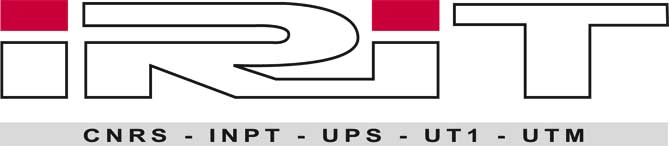
\includegraphics[scale=0.1]{irit}
\lfoot{Three-dimensional modeling and printing}}
\rfoot{\thepage}

% Code
%\usepackage{minted}

\begin{document}

\bigskip
\bigskip
\bigskip
\bigskip
\bigskip
\bigskip
\bigskip
\bigskip

\begin{center}
\huge{Three-dimensional modeling and printing:\\ Project report\\}
\bigskip
\bigskip
\Large{from January 23 to March 16, 2012}
\end{center}

\bigskip
\bigskip

\begin{center}
\large{
\textit{Vincent \textsc{Duvert} \\
Antoine \textsc{Lubineau} \\
Caroline \textsc{Naud} \\
James \textsc{Packer} \\
Florian \textsc{Ribon}} \\
\bigskip
INP-ENSEEIHT/IMA 
}
\end{center}

\bigskip
\bigskip

	This report summarizes the context, the organization, the work and the outcomes within the 3D modeling and printing project suggested by the VORTEX team of IRIT to third-year students in the IMA department of ENSEEIHT.

\bigskip
\bigskip

\begin{figure}[!h]
\begin{center}
	
\includegraphics[scale=0.4]{inp-enseeiht}
\end{center}
\end{figure}

\bigskip

\begin{center}
\url{http://www.enseeiht.fr/fr/index.html} \\
2 Rue Charles Camichel \\
31 071 TOULOUSE
\end{center}

\vfill

\begin{figure}[!h]
\begin{center}
	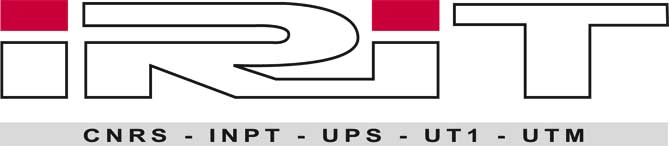
\includegraphics[scale=0.4]{irit}
\end{center}
\end{figure}

\begin{center}
\url{http://www.irit.fr}\\
Université Paul Sabatier \\
118 Route de Narbonne \\
F-31062 TOULOUSE CEDEX 9
\end{center}

\thispagestyle{empty}

\newpage

\chapter*{Acknowledgments}
\addcontentsline{toc}{chapter}{\numberline{}Acknowledgments}

	Our most sincere thanks go to our technical supervisor, Lionel \textsc{Cremel}, for guiding us throughout this two-months project and having initiated us in a progressive and efficient way to the art that is project management. Our project would certainly not have got the same results without him.\\

\bigskip

	We also want to thank Axel \textsc{Carlier}, Jean \textsc{Conter} and Géraldine \textsc{Morin} for having proposed such an interesting subject and for all the help and the pieces of advice they have been giving us during the project.\\

\bigskip

	We also thank all the people we have met during our visits to the manufacturing laboratory \href{http://artilect.fr/}{Artilect} who got interested in our project and agreed to share with us their expertise in this area, as well as Alexandre \textsc{Girard} from \href{http://tetalab.org/}{Tetalab} with whom we exchanged practical information on the Ultimaker printer.


\tableofcontents

\chapter{Presentation of the project}

\section{The context}

	The \textit{3D printing} phrase is used to describe the process of creating three dimensional objects from digital files using a materials printer in a manner similar to printing images on paper. The term is most closely associated with additive manufacturing technology, where an object is created by laying down successive layers of material.\\

	Since 2003 there has been a large growth in the sale of 3D printers since the technology actually finds use in more and more fields such as jewellery, footwear, industrial design, architecture, engineering and construction, automotive, aerospace, dental and medical industries, education, geographic information systems, civil engineering, and many others.\\

	The VORTEX team (Visual Objects : from Reality To EXpression) from IRIT (Institut de Recherche en Informatique de Toulouse) is part of the numerous people having found interest in this technology and recently acquired an Ultimaker 3D printer which she did not have the time to calibrate and that she would like to be able to use in order to print 3D mono-color objects. To that end, she would need to be able to create, model and edit these objects within a software (to be conceived or modified) using, if possible, the multi-touch screen she already owns (Acer T231H).\\

\section{The final users of the product}

	The primary final users of the 3D modeling software and of the printer would be the researchers of the team of IRIT. However, they really aim at offering this service to artists, such as those already using an Ultimaker 3D printer in the Fablab in Toulouse.

\section{The work required}

	The project was divided into two major parts. The first consisted in developing an open-source software with graphical interface that could allow to model and deform virtual 3D objects, preferably using a dual-touch screen. The second part concerned the export of this object (as a mesh) to the printer to finally print it as realistically as possible.

\section{Available resources}

\subsection{The project team}

	Our team was composed of five students from the Computer Science and Applied Mathematics department of ENSEEIHT who all showed a real interest in the subject. These people are listed here:

\begin{itemize}
	\item Caroline \textsc{Naud}: project manager
	\item Vincent \textsc{Duvert}
	\item Antoine \textsc{Lubineau}
	\item James \textsc{Packer}
	\item Florian \textsc{Ribon}
\end{itemize}

\subsection{Material resources}

	We list below all the material resources which were available to us during the project:

\begin{itemize}
	\item the room F117 in building F at ENSEEIHT (same building that the one the \textsc{VORTEX} team works in
	\item an Ultimaker 3D printer with a roll of PLA plastic
	\item a computer with a dual-touch screen Acer T231H
	\item all computer rooms of ENSEEIHT
	\item our personal computers
\end{itemize}

\chapter{Project management}

\section{Project supervision}

	During the first week of the project we were introduced to Lionel \textsc{Cremel}, project manager at \textsc{Airbus}, who had volunteered to guide us in managing our project. We agreed on that day to meet him at least once a week nearly every week so that he could guide us throughout the project. We give here the dates on which we successively met and the main content of the meetings:
	
\begin{itemize}


	\item Week 1 (January, 24): introduction of the project members, choice of the project management model, introduction of the specification phase of the V model
	\item Week 2 (January, 27): choice of the project manager
	\item Week 3 (February, 6): evaluation planning, risks assessement
	\item Week 4 (February, 9): start of development phase
	\item Week 5 (February, 20): progress update, client meeting planning, risks assessement
	\item Week 6 (February, 29): planning of testing phase, client meeting report
	\item Week 7 (March, 7): testing phase results, documentation writing planning

\end{itemize}

On each meeting, Lionel successively explained us how to decide of a macroscopic planning for our project, told us about the different milestones they use in Airbus projects and the documents that should sometimes be available when arriving at a milestone and guided us throughout the management of our human and material resources. Of course, we couldn't do exactly as he was used to do Airbus (simply because our project is happening in quite special conditions) but thanks to that, we could have a real idea of what project management would be in the future. 

\section{Resource management and planning}

With the help of Lionel, we all agreed on saying that a V-cycle was adequate for the progress of our project. This cycle includes (as shown on the picture below):

\begin{itemize}
	\item a specification part (requirements, design and architecture) in which the final user tests and the functional tests are decided,
	\item an implementation part in which unit tests are run on the different functionalities implemented,
	\item a validation phase in which all the tests are run and at the end of which a final acceptance should be obtained from the client.
\end{itemize}

\begin{figure}[!h]
\begin{center}
	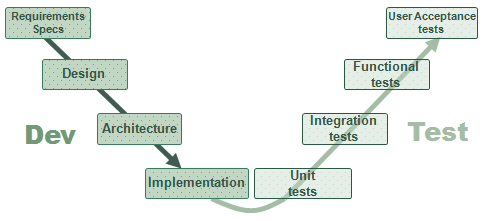
\includegraphics[scale=4.5]{VCycle}
\end{center}
\end{figure}

However, our project was special and could not totally follow that scheme since it contained a part on which we had to learn how to use the printer and which were the adapted parameters to get good quality objects. We thus thought that this part deserved to have at least one member of the team dedicated to it at full time. This member would of course participate in the rest of the project but would spend most of his time on the printer. The four other members would equally participate in all the different steps of the project. Three of us would use their personal computers while the last one would sometimes work from his place or from the computer room at ENSEEIHT and would sometimes use the computer made available to us by the client team. This last one would also often be used by the student dealing with the printer to pilot it.\\

The macroscopic planning we chose is given here:

\bigskip
\begin{figure}[!h]
\begin{center}
	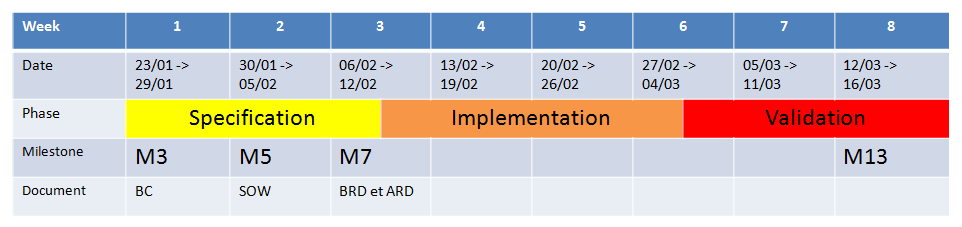
\includegraphics[scale=0.4]{PlanningMacroscopique}
\end{center}
\end{figure}

As shown here, we decided to give approximatively the same time to each main part of our project, this is to say 2 to 3 weeks. The first main phase is here the only one containing milestones. This is because these were quite the most important milestones to us. They corresponded to the main documents we had to produce before starting the development. These documents will be given later in this report. They had to be submitted to the client so that we would be totally sure that we add completely understood their need.\\

A more detailed planning containing the different tasks we achieved is available in the appendix and will be explained in the rest of this report.

\section{The risks assessment}

Our supervisor also taught us how to manage the possible risks in our project so that we would not have any delay of major issues which would prevent us from delivering a good quality product. This work included the detection of theses risks, the finding of a way to prevent them and a mitigation if they would still happen. Of course, this assessment changed as time went by since some of the risks disappeared or actually happened and new appeared.

We give here an example of this assessment we did on our second week of work:

\begin{center}
	\begin{tabular}{|p{4cm}|p{5cm}|p{5cm}|}
		\hline
		Category & Risk & Prevention solution \\ \hline
		Material resources & Printer failure & Warn the Fablab that we could use their printer, use ours with caution \\
		Documentation & Lack of documentation & Ask the teachers for help \\
		Client's needs and specifications & Late change in the customer's expectations & Tell them we won't accept any change after a certain date \\
		Project management & Not enough slack & Include consequent slacks in the planning \\
		Tests and deployment & Ineffective tests & Plan enough time to prepare relevant tests \\
		Quality & Disagreement between the needs and the solution & Organize as many meetings as possible with the client \\
		Technical risks on development & Bad modeler choice & Plan enough time to pick the best solution possible \\
		\hline
	\end{tabular}
\end{center}

\chapter{The specification phase}

This was the first main phase of our project. Our main goal at the end of this phase (on February, 12th) was to fully determine with the client the specifications of the project so that we would change them as little as possible. The achievement of this goal included to first understand what the client team expected from us on a general way (Statement Of Work) to them detail these needs and find technical solutions to satisfy them. This phase thus implied regular meetings with the client team.

\section{The establishment of the Statement Of Work}

We first met the client team on January, 20th when they completely presented us the project for the first time. One of us was missing that day because still in semester abroad but we managed to tell him all about that meeting afterwards.\\

The client team first told us about this Ultimaker 3D printer she recently acquired and which she did not have time to calibrate. Our main goal at that time was to clearly establish the clients' needs but we quickly discovered they did not have an exact idea of what they wanted to do with that printer, apart from printing meshes they would have previously had modeling interactions with.\\

They also mentioned later that they wanted to be able to know, before printing it, that a mesh was not correct. Considering the time we had, we later decided we could even try to correct the meshes instead of simply highlighting its defaults. \\

Finally, they told us about the documentation they needed to be provided with so that they could use and modify our work later. \\

We must notice that our project was quite atypical considering the fact that, even though we had planned to have fully decided on the specifications on February, 12th, our clients kept asking us about what could be useful until the last day.

\section{The general architecture of the project}

As we all started to discover the printer, it came to us that the final application would include the use of several software. Indeed, the use of the printer first implies the transformation of the mesh created with the modeler into instructions for the printer (G-code) which we then need to send to the printer previously parametrized. This makes the 4 main parts given in the following figure:

\bigskip

\begin{figure}[!h]

\begin{center}
	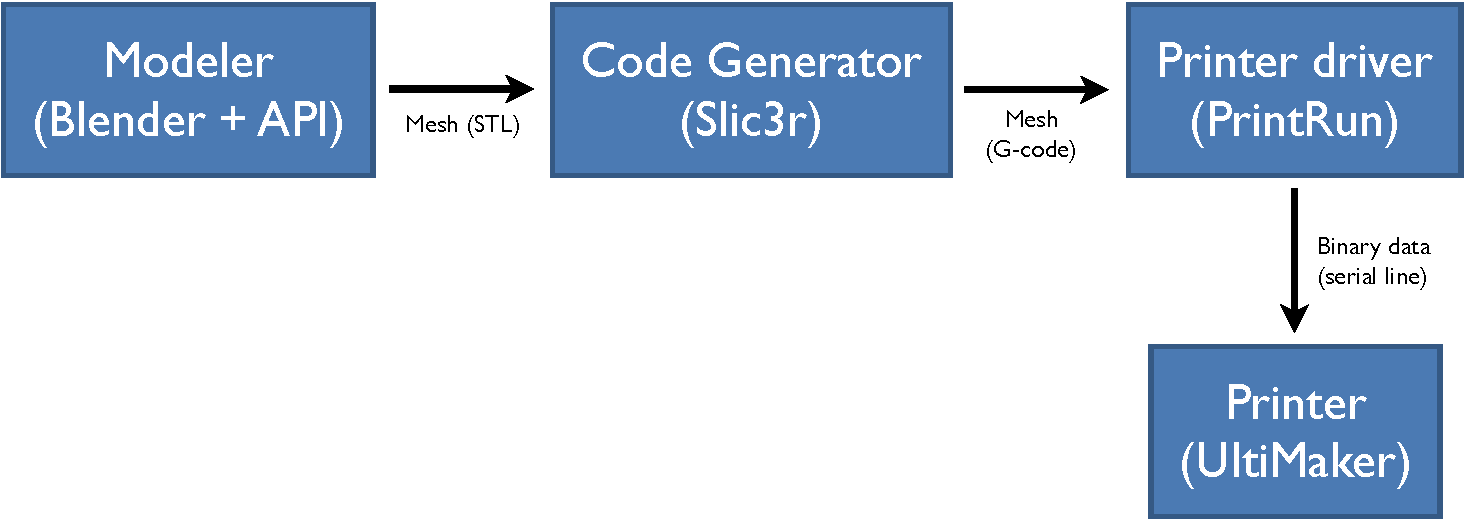
\includegraphics[width=.7\textwidth]{schema}
\end{center}

\end{figure}

We decided not to act on the printer's firmware (although it is possible to do so), and to focus on the modeler, the G-code generator and the printer driver. These choices are explained later in this report. 

\section{The redaction of the technical specifications}

One we had determined the clients' needs, we had to specify exactly what would be integrated into our application. The initial technical requirements are listed below.

\subsection{Modeler}

\bigskip

\begin{enumerate}
	\item Create, model and edit 3D objects on Windows and Linux:
	\begin{enumerate}
		\item STL and PLY import from the computer
		\item STL export to the G-code generator
		\item Directly deform meshes:
		\begin{enumerate}
			\item Add, remove, translate a vertex
			\item Smooth a surface (automatically add faces, etc.)
			\item Cut an object
			\item Handle the case of several objects (multiple verifications, multiple exports)
		\end{enumerate}
	\end{enumerate}
	\item{Check mesh printability:}
	\begin{enumerate}
		\item Check if the mesh is manifold and fill it if not
		\item Check if the mesh is watertight
		\item Check if the orientation is good for printing:
		\begin{enumerate}
			\item Report a bad supporting plan
			\item Suggest a good supporting plan
			\item Suggest to add a platform to the object if there is no adequate supporting plane
		\end{enumerate}
	\end{enumerate}
	\item{Provide a simple and easy to use interface:}
	\begin{enumerate}
		\item Provide an adequate layout for mesh interaction and verification
		\item Automatically verify the printability of a mesh (either in reaction to events, periodically or on demand)
	\end{enumerate}
\end{enumerate}

\bigskip

What must be said is that some of these requirements were not directly expressed by the client team but were suggested by us (because the client had not thought about them and because we planned we would have time to integrate them). That's why they are not exactly implemented as expressed but in a quite different way. This is due to the fact that, while progressing in our work, we had new ideas about how to integrate these notions in Blender. All these reflexions are detailed later in this report.

\subsection{Printer}

Find the adequate printing parameters, depending on the kind of object printed.

\subsection{Documentation}

\begin{enumerate}
\item produce a user documentation: to use the application properly just by reading it. It should include the limits of the application.
\item generate a technical documentation: so that the client or an other team can continue the work if needed
\item write an installation paper: to enable the user to get an operational application from the initial archive
\end{enumerate}



\section{The technical choices}

\subsection{Choice of the modeler}

Developing a 3D modeler ``from scratch'' would have needed a considerable amount of time. That's the reason why we chose to start from an existing modeling program since many where already existing and already contained some of the features we needed.\\

Since we needed to provide the client team with a fully open-source application, we decided to list all the existing modelers we found and to weight up their pros and cons. After a few day, our choice was reduced to the two following modelers \emph{Meshlab}\footnote{\url{http://meshlab.sourceforge.net/}} and \emph{Blender}\footnote{\url{http://www.blender.org}}. We give here the drawbacks and advantages we highlighted for each one and explain our final choice.

\bigskip

\bigskip

\fbox{\begin{minipage}{0.9\textwidth}

\textbf{Blender :}\\

\underline{Advantages :}

\begin{itemize}
\item many of the requested features already present
\item existence of a Python API allowing the integration of personal scripts
\item required formats well managed (STL and PLY)
\item interface easily adaptable
\end{itemize}

\underline{Drawbacks :}

\begin{itemize}
\item a lot of useless functionalities for the project final users
\end{itemize}

\end{minipage}}

\bigskip

\fbox{\begin{minipage}{0.9\textwidth}

\textbf{Meshlab :}\\

\underline{Advantages :}

\begin{itemize}
\item STL format well managed
\item easy use
\item only essential functionalities
\end{itemize}

\underline{Drawbacks :} 

\begin{itemize}
\item almost no preexisting interaction
\item need to learn to program with C++ ...
\end{itemize}


\end{minipage}}

\bigskip

\bigskip

We finally chose to use \emph{Blender}, and modify it to fit our needs. Instead of modifying the Blender core code, we chose to write Python modules implementing our added functionalities. The Python\footnote{\url{http://www.python.org}} programming language provides some programming facilities (automatic memory management, for instance) which ease the implementation of algorithms.

\subsection{Choice of the GCode Generator and of the printer's pilote}

\chapter{The implementation phase}

\section{The mesh correction - \textit{Florian \& James}}

We have implemented a script which allows the user to track broken, non-manifold edges on the working object in Blender, and offers him two different ways to correct them.\\

First of all, a press on the Check button (see the GUI modification part) highlights all the potential non-manifold edges and gives the user the possibility to repair them if the mesh is actually non-manifold.\\

The first method is a soft correction algorithm, which detects all distinct holes in the mesh, then cleans theses holes (for instance if there are some faces not connected to any vertex), and finally try to fill them, one after one. This method is considered non-destructive (even if the cleaning part may remove unwanted faces) and is not recursive. The algorithm has been proved to make a broken mesh watertight, so there is no more holes remaining after its execution.\\

But even if it is watertight, a mesh may still remain non-manifold. Therefore, we implemented a strong correction algorithm which is able to repair all kinds of edges-related problems. This strong destructive method consists in a loop of soft correction calls, with a selection and removal of remaining non manifold edges (and thus which didn't belong to any standard hole) between each iteration. By properly removing these edges, new holes appear and the next iteration will try to fill them the correct way. Eventually, the mesh is fully manifold (thus watertight).\\

For both the destructive method and the non-destructive one, we added a fast-processing option which makes the correction algorithms way faster than without enabling it. But activating it may result in various artifacts between some edges. Since it works better on bigger and well-detailed objects (with finer meshes), the user should try to use it first on big objects and if the result is not satisfying, he simply has to cancel the last operations and then try again with the fast-processing check box disabled. This option only acts during the holes filling action, by trying to fill all of them with only one single filling call, while the standard option requires another algorithm which we developed and which detects and separates all distinct holes within the mesh.


\section{The choice of the supporting plane - \textit{Antoine \& Vincent}}

\subsection{The supporting planes auto-detection}
Before being printed, the objects need to be placed correctly; they have to stand on the the printer’s support. From the modeler point of view, the object need to have faces included into the base ($z = 0$) plane, and may not have any points under this base plane. We need to provide the user an automated way to correctly place the object.

Correct positioning is not enough, though. The object support must be large enough for the object to be stable during printing; some gravity center considerations may also be taken into consideration.

The first algorithm we developed finds “supporting planes” for an object. It works in multiple steps:
\begin{enumerate}
\item Cluster faces belonging to the same plane. This is done by first comparing the angle between the normals of the two faces. If it is close to $0$, the faces have approximatively the same orientation; we then need to check if they are on the same plane. This is done by picking a point of each face and projecting both on the common normal of these two faces. If the projections are equal, we assume that the two faces are in the same plane, and they are placed in the same cluster.
\item The planes defined by the face clusters may cut the object in half; we want to filter out these clusters and only provide the other clusters to the user. We start by defining, for each cluster, the corresponding plane: we define it by a point and a normal. We then check that every point of the object is on the “right” side of the plane: this is done by projecting the points on the plane’s normal, and checking that the projection result is lower than the plane’s point own projection on the normal. If every point passes the test, the plane is accepted as a supporting plane.
\end{enumerate}

Since the bigger supporting surfaces are preferred, we provide the user the 10 largest surfaces found (this number may be changed in the Python script), in decreasing order of area. When a supporting surface is selected, we need to correctly orient the object (rotation + translation) so it stands on this surface.

\begin{itemize}
\item The rotation to apply is the one which transform the chosen plane’s normal into the base plane’s normal (which is $(0, 0, -1)$).
\item The translation to apply is the one which places the chosen plane’s point into the base plane: we just need to take this point’s $z$ and apply a translation of $(0, 0, -z)$ so this point’s new coordinates are $(x, y, z=0)$.
\end{itemize}

\subsection{The user-helped face selection / object cutting}
The above system is helpful for a large variety of objects, but may not work correctly for ones without large ``exterio'' supporting planes. In that case it is needed to cut some parts of the object. To facilitate these operations, two features are provided.
\begin{itemize}
\item The first one simply cuts all parts of the object which are under the base plane. This operation is done by using Blender’s ``boolean difference'' operation between the object and a rectangular parallelepiped of the correct size (placed under the base plane).
\item The second one asks the user to select some faces of the object. Those faces are used to calculate a supporting plane (possibly cutting the object in half) which is the used to position the object. The parts of the object under the base plane are then removed.
\end{itemize}

\subsection{The socle generation}
Finally, another feature allows the automatic generation of a ``socle'', which can support the object. This is done by adding a socle (rectangular parallelepiped of the correct size) and merging it to the object (using a ``boolean union'' operation).

\section{The GUI modification - \textit{Caroline}}

Although we had decided to work on Blender, its graphic interface remained quite difficult to use for inexperienced users and still showed ``useless'' functions. \\
While making researches about Blender, we discovered that we could manually modify its graphic interface as we wanted to only keep the most useful features visible. This was done while drag 	and dropping some windows and panels. We then registered the corresponding file (\textit{startup.blend}) to have it to the adequate place in the final product. We give here the the interface we configured :

\bigskip
\bigskip

\begin{figure}[!h]
\begin{center}
	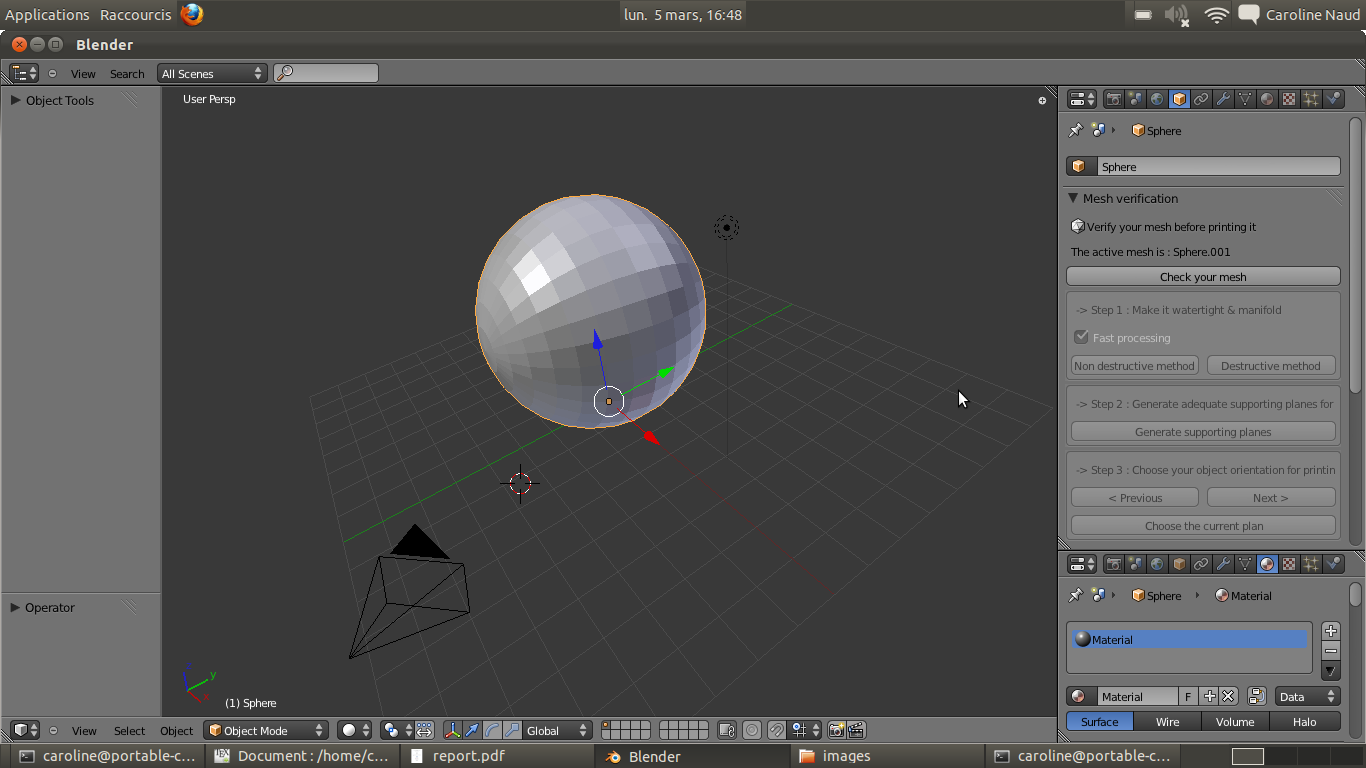
\includegraphics[scale=0.3]{NotreInterface}
\end{center}
\end{figure}

\bigskip
\bigskip

We only chose to keep visible what was necessary to the final user simply wanting to impport, modify and correct a mesh.\\

The part we see at the right of the screen and which seem a little grey is the panel we added so that the user can have access to the different functions we implemented. It was also coded thanks to the Blender Python API which allows to create buttons, check boxes ... The panel is visible next page.

\newpage

\bigskip
\begin{figure}[!h]
\begin{center}
	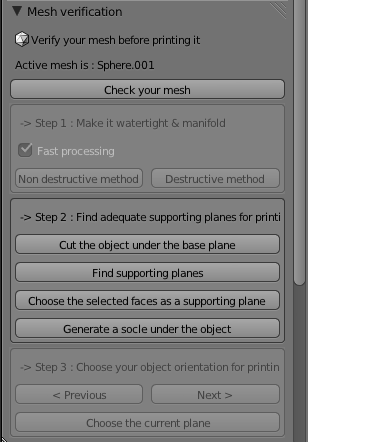
\includegraphics[scale=1]{Panel}
\end{center}
\end{figure}
\bigskip

As for the organization of the Mesh Verification panel, we chose to divide if into 4 main parts that we called ``steps'' since we considered that the the user would have to use them successively. We detail these steps here below.\\

\textbf{Step 0 : not written on the panel} \\

This part of the panel remind the user of the active mesh in the scene. It is also the first and only enabled button in the panel when starting Blender. It is to be used when the mesh is satisfying for the user to check if it is correct or not (manifold and watertight). By passing the mouse over the button, a description of the action is given, as for all the buttons and check boxes. When pressing this button, the script of verification will be run and it outcome will determine the next step enabled. If the mesh is found incorrect, the user will see the first step enabled and only this step. If it is found correct, the second step will be enabled.\\

\textbf{Step 1 : the mesh correction step} \\

This step enables a check box and two different buttons allowing the user to correct the mesh the way he wants and in a chosen time (see the mesh correction part). When the mesh is considered correct by the script run when pressing the buttons, the step 2 is enabled.

\textbf{Step 2 : the finding of an adequate supporting plane for printing}\\

This step has been realized so that the user can both trust the application to find an adequate supporting plane for his object and decide of the supporting plane himself. \\

This last possibility is included in the ``Cut the object under the base plane'' button. This button allows the user to plane his object himself where he wants be orienting it and positioning it considering the $z = 0$ plan. This can be useful when printing an egg for example. In this case, there is no plane to support the object. Another button enabling the user to choose the supporting plan himself is the third one when he can select one and choose it so that the object will be automatically oriented as chosen.\\

But in this step, the user can also trust the scripts implemented to find several adequate supporting planes on the object (the number of planes generated being chosen by the developer). When this button is pressed, the ``best'' plane found according to the script is highlighted and the third step is enabled to choose between all the other planes.\\

\textbf{Step 3 : the choice between the generated planes}\\ 

In this step, planes have previously been found to support the object and the ``Next'' and ``Previous'' buttons allow the user to navigate among them, highlight them and select one for supporting the object. Once the ``Choose the current plane'' button is pressed, the step 0 is enabled again while the third one is disabled. 

\chapter{The printer calibration}

\chapter{The validation phase}

\section{Unit tests}

\section{Integration tests}

\section{Functional tests}

\section{User tests}

\section{The application's limitations}

\chapter{Conclusions}

\addcontentsline{toc}{chapter}{\numberline{}Bibliography}

\appendix

\end{document}
